\chapter{Vistas de la arquitectura no implementadas}
\label{app:vistas_no_implementadas}

A continuación son mostradas las vistas creadas por los autores pero que no son utilizadas para el desarrollo de las funcionalidades del presente prototipo.

\section{Business Functions Viewpoints}

\subsection{Patrocinios Deportivos}

\begin{figure}[!htb]
  \begin{center}
    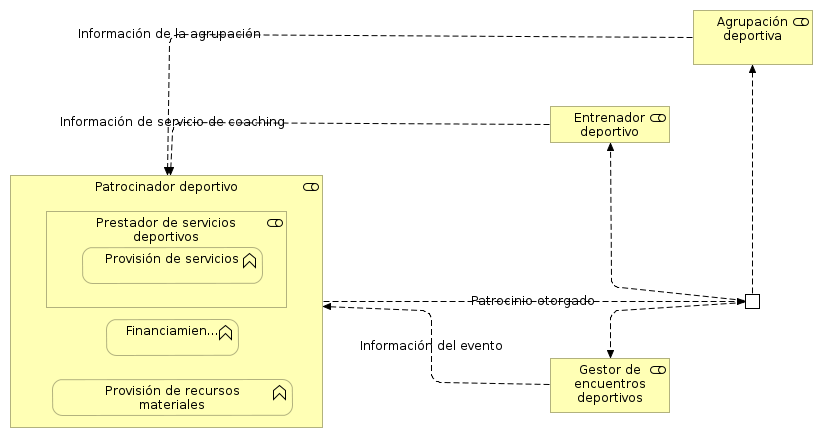
\includegraphics[width=11cm]{./imagenes/Archimate/vistas/business_functions/patrociniosdeportivos.png}
    \caption{Patrocinios Deportivos}
    \label{fig:bf_patrocinios_deportivos}
    \textbf{Fuente:}  Autores
  \end{center}
\end{figure}

En este punto de vista se puede observar cómo los patrocinadores pueden patrocinar diferentes actores en la red social. Más a fondo, se puede ver como un patrocinador apoya los proyectos desempeñados por un actor que desempeña un rol específico en la red social. Así, por ejemplo, un gestor de encuentros deportivos puede pedir un patrocinio o recibir una petición de un patrocinador para ser patrocinado por el evento que va a realizar. También se puede observar que un patrocinador deportivo patrocina proyectos de otros actores sobre la red social con su financiamiento, con la prestación de uno o varios servicios o con la provisión de uno o varios recursos materiales.

\subsection{Formación de Grupos Deportivos}

\begin{figure}[!htb]
  \begin{center}
    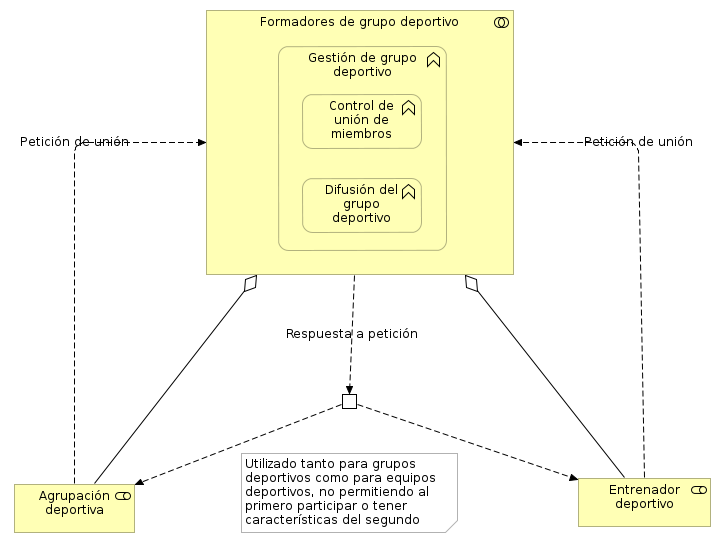
\includegraphics[width=11cm]{./imagenes/Archimate/vistas/business_functions/formaciongruposdeportivos.png}
    \caption{Formación de Grupos Deportivos}
    \label{fig:bf_formacion_grupos_deportivos}
    \textbf{Fuente:}  Autores
  \end{center}
\end{figure}

En cuanto a la formación de grupos se refiere, entre roles intercambian la información acerca de sus peticiones a unirse a la red social, así como la respuesta a la misma. Se puede ver que los roles que interactuan en la formación de grupos deportivos son solo los de entrenadores y agrupaciones deportivas y que ellos mismos conforman los grupos deportivos.

\subsection{Entrenamiento Deportivo}

\begin{figure}[!htb]
  \begin{center}
    \includegraphics[width=11cm]{./imagenes/Archimate/vistas/business_functions/entrenamientodeportivo.png}
    \caption{Entrenamiento Deportivo}
    \label{fig:bf_entrenamiento_deportivo}
    \textbf{Fuente:}  Autores
  \end{center}
\end{figure}

Sobre este punto de vista se puede observar el flujo de información entre los roles participantes en un entrenamiento deportivo. Todos están basados en la valoración del trabajo producido en la práctica según los eventos producidos en la misma y la valoración que a estos de cada rol para, así, producir ejercicios deportivos para el entrenamiento.

\section{Business Process Viewpoints}

\subsection{Patrocinios Deportivos}

\begin{figure}[!htb]
  \begin{center}
    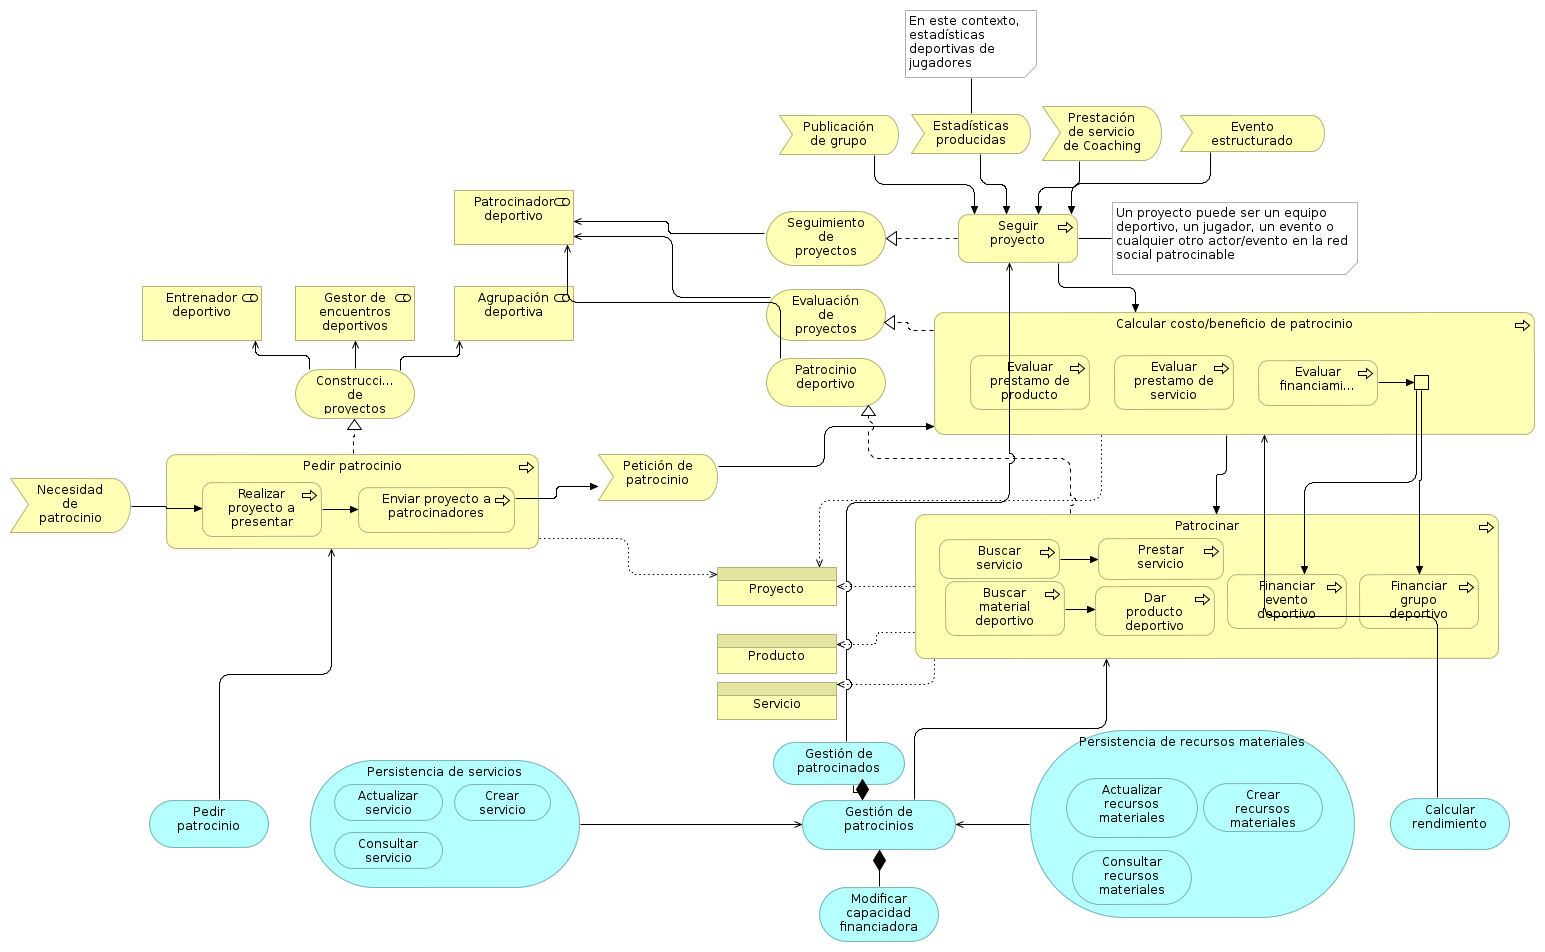
\includegraphics[width=11cm]{./imagenes/Archimate/vistas/business_process/patrociniosdeportivos.png}
    \caption{Patrocinios Deportivos}
    \label{fig:bp_patrocinios_deportivos}
    \textbf{Fuente:}  Autores
  \end{center}
\end{figure}

En el proceso de patrocinios, los autores han orientado el proceso de negocio partiendo desde el patrocinado hacia el patrocinador (con la petición de patrocinios) y desde el patrocinador al patrocinado (dejando al patrocinador decidir si patrocinar o no un proyecto según el seguimiento que él le haga a éste). Se puede ver también que los servicios ofrecidos soportan todos los procesos de negocio ilustrados.

\subsection{Formación de Grupos Deportivos}

\begin{figure}[!htb]
  \begin{center}
    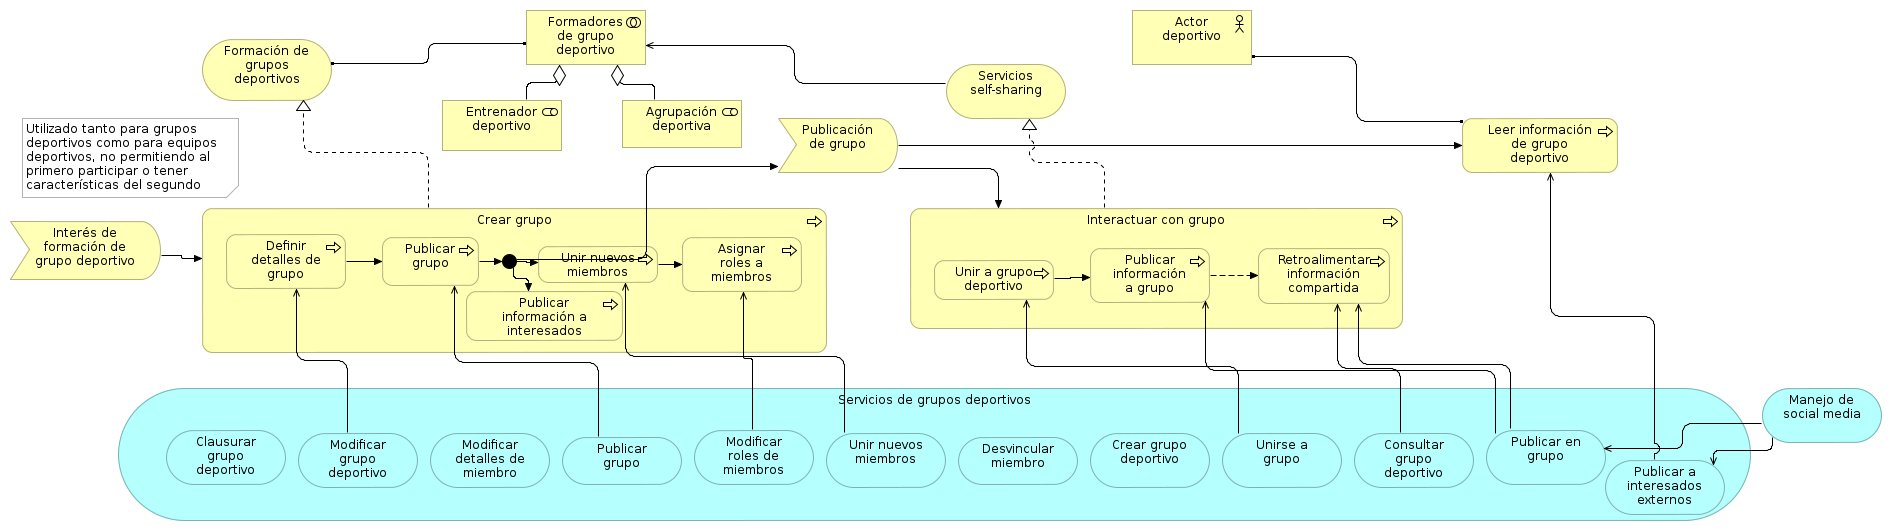
\includegraphics[width=11cm]{./imagenes/Archimate/vistas/business_process/formaciongruposdeportivos.png}
    \caption{Formación de Grupos Deportivos}
    \label{fig:bp_formacion_grupos_deportivos}
    \textbf{Fuente:}  Autores
  \end{center}
\end{figure}

Este punto de vista de proceso de negocio está basado en dos procesos principales: La creación de un grupo deportivo y la interacción con el grupo deportivo. Lo que los arquitectos transmiten es el cómo, luego de la creación del grupo, se desempeñan procesos que luego serán recurrentes a través de la vida del grupo deportivo: La interacción grupal y la asignación de roles sobre integrantes del grupo deportivo. Según el punto de vista, solo aquellos con rol de entrenadores deportivos y de agrupaciones deportivas pueden formar un grupo deportivo. Hay un tercer proceso que es la lectura de información del grupo deportivo, en el caso de un actor deportivo que esté interesado en unirse/participar en el grupo deportivo. Este punto de vista es utilizado tanto para grupos deportivos como para equipos deportivos, no permitiendo al primero participar o tener características del segundo.

Los procesos de negocio representados son cubiertos por un servicio grande específico para prestar funcionalidades a los grupos deportivos y éste, a su vez, hace uso del servicio de social media para poder implementar la interacción grupal.

\subsection{Entrenamiento Deportivo}

\begin{figure}[!htb]
  \begin{center}
    \includegraphics[width=11cm]{./imagenes/Archimate/vistas/business_process/entrenamientodeportivo.png}
    \caption{Entrenamiento Deportivo}
    \label{fig:bp_entrenamiento_deportivo}
    \textbf{Fuente:}  Autores
  \end{center}
\end{figure}

El proceso de entrenamiento deportivo ha sido dividido en dos procesos grandes, uno atado al entrenador solamente (entrenar grupo deportivo) y otro atado tanto a la agrupación deportiva como al entrenador deportivo (ejecutar plan de entrenamiento). Sobre estos dos grandes procesos se destacan las funciones expresadas en el punto de vista de funciones de negocio de entrenamiento deportivo. Sobre esta vista se manejan dos objetos de negocio principales: evaluaciones deportivas y planes de entrenamiento.

En función de soportar los procesos expresados por los autores, se generaron tres servicios de aplicación principales: La ejecución de un plan de entrenamiento, otros servicios de gestión del plan de entrenamiento y un servicio para el soporte de la evaluación deportiva, el cual se nombró "servicio de comunicación colaborativa".

\section{Application Usage Viewpoints}

\subsection{Patrocinios Deportivos}

\begin{figure}[!htb]
  \begin{center}
    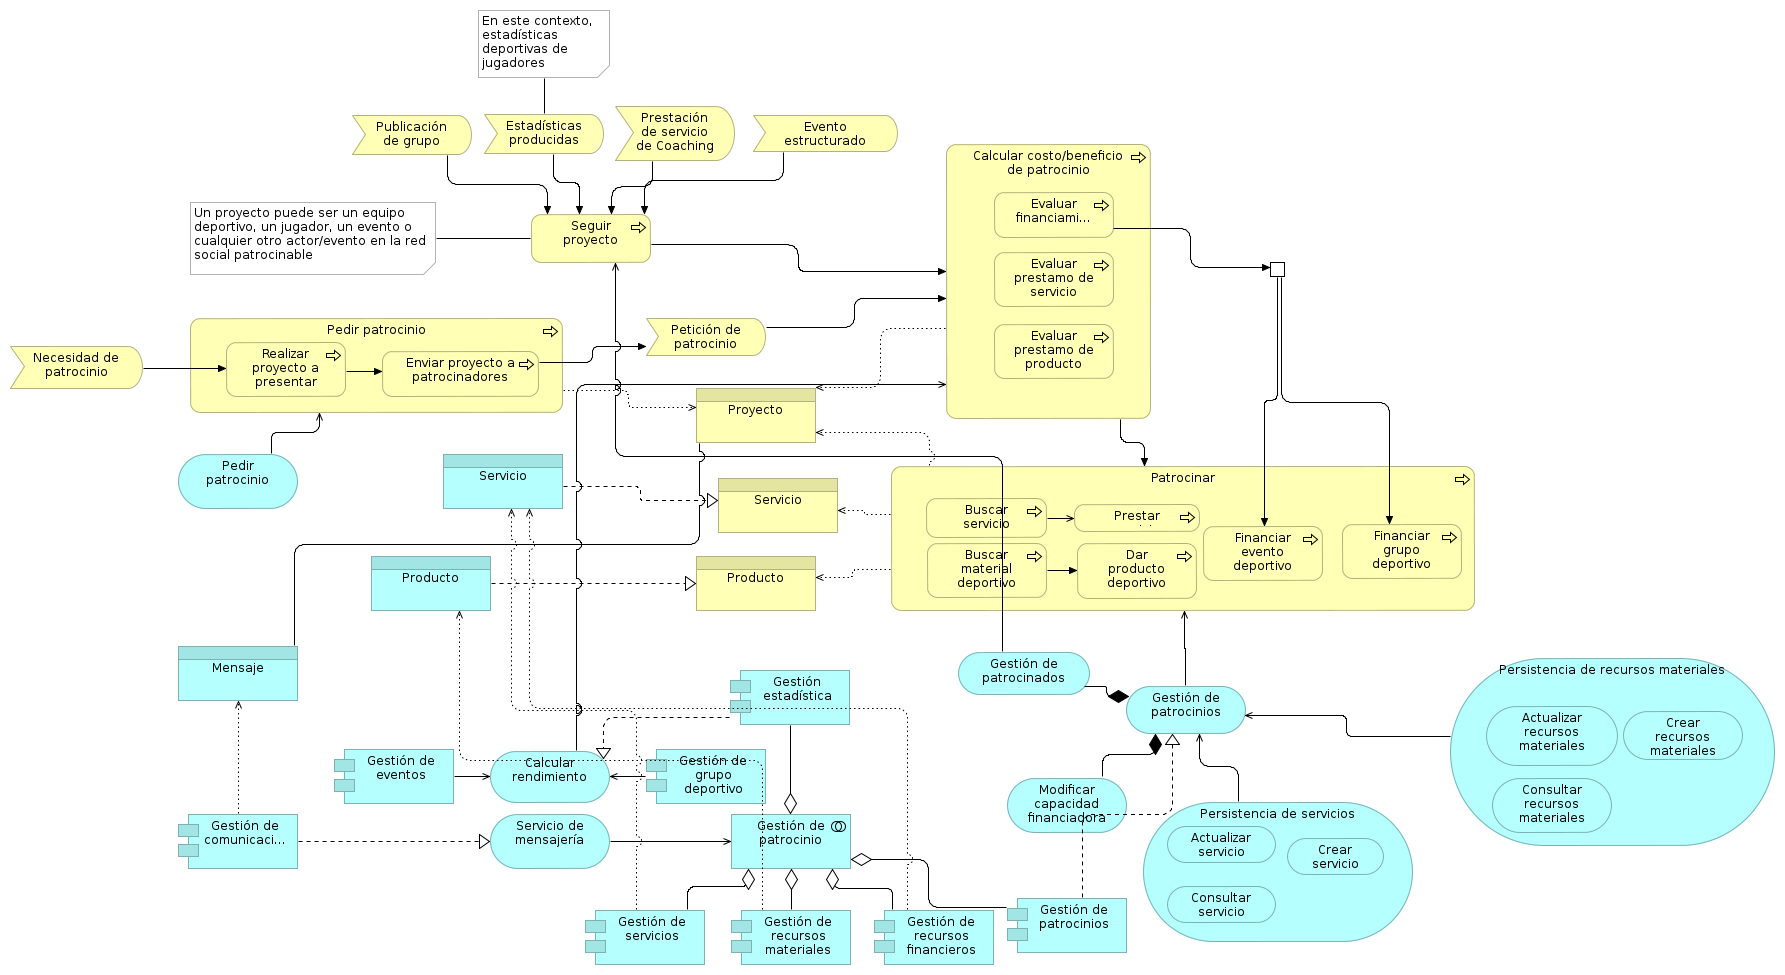
\includegraphics[width=11cm]{./imagenes/Archimate/vistas/application_usage/patrociniosdeportivos.png}
    \caption{Patrocinios Deportivos}
    \label{fig:au_patrocinios_deportivos}
    \textbf{Fuente:}  Autores
  \end{center}
\end{figure}

A parte de lo ya observado en el punto de vista de proceso de negocio de patrocinios deportivos, en este punto de vista puede observarse con los objetos de negocio, en particular, que en la aplicación el objeto de negocio "proyecto" no va a ser soportado más que como un posible paso de mensajes entre patrocinador y patrocinado, puesto que el servicio que soporta el proceso de negocio de petición de patrocinios sólo envía la intención de ser patrocinado como un mensaje, en otras palabras, el SNS no soporta la creación de proyectos aunque si facilita la visualización de factores que influyen en el patrocinio de un actor deportivo (como, por ejemplo, las estadísticas deportivas generadas para un actor deportivo).

Se hace la creación de componentes de negocio para la gestión de cada facilidad ofrecida por un patrocinador, así como también uno para el patrocinio mismo, gestión de patrocinios, soportando los servicios de patrocinio ofrecidos. La utilización de los demás servicios se ve reflejada en componentes relacionados con estadísticas, con grupos deportivos y con eventos deportivos. También se observa un componente de comunicación, el cual realiza el servicio de mensajería para el envío de mensajes (proyecto) entre patrocinador y patrocinado.


\subsection{Formación de Grupos Deportivos}

\begin{figure}[!htb]
  \begin{center}
    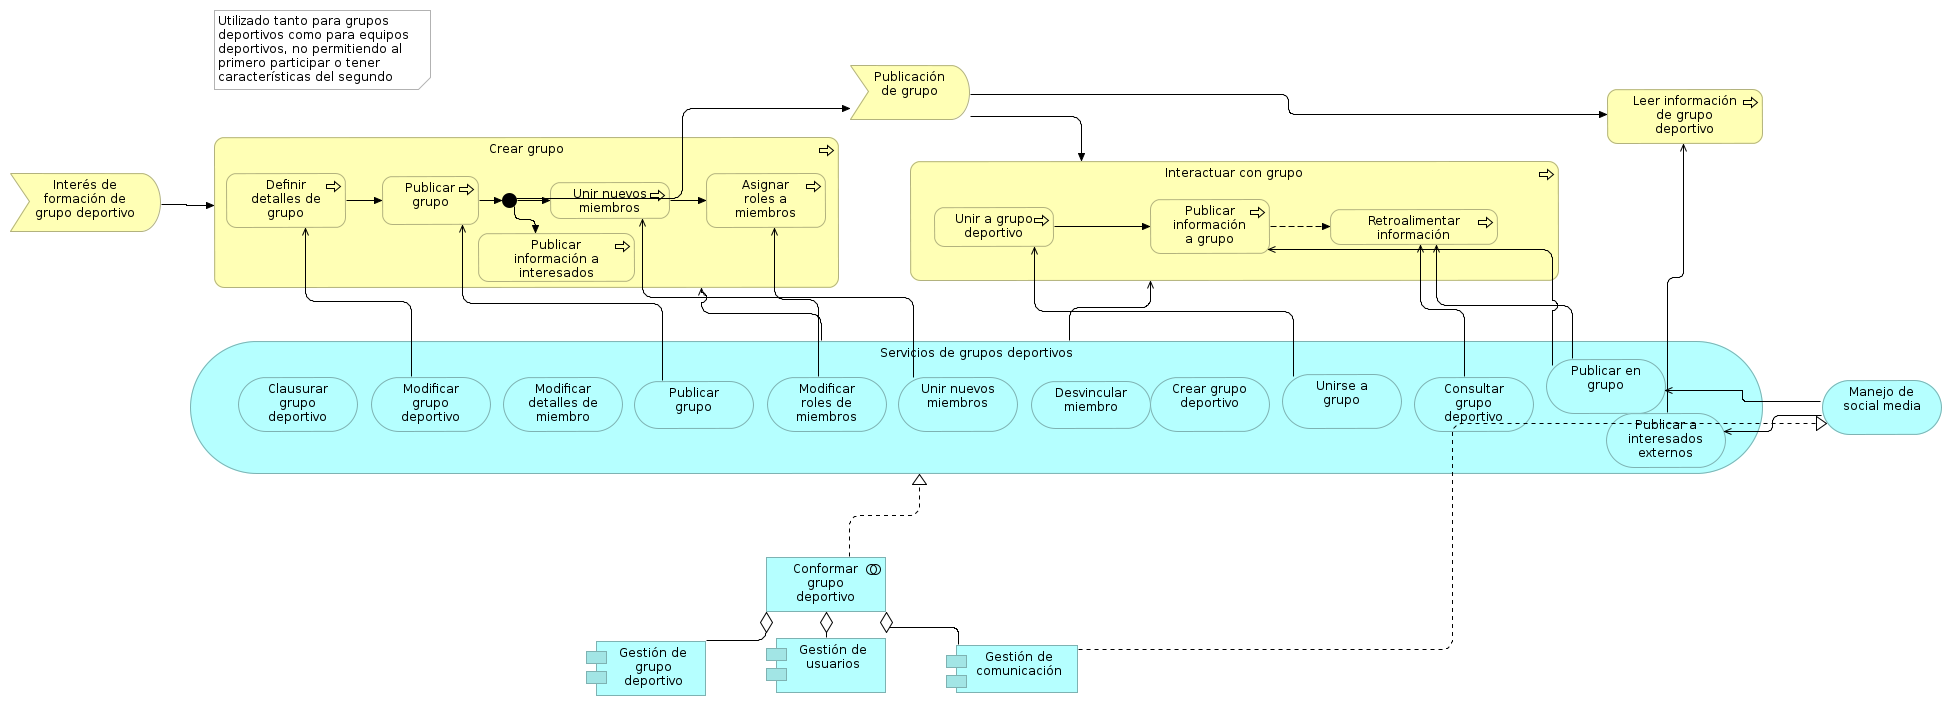
\includegraphics[width=11cm]{./imagenes/Archimate/vistas/application_usage/formaciongruposdeportivos.png}
    \caption{Formación de Grupos Deportivos}
    \label{fig:au_formacion_grupos_deportivos}
    \textbf{Fuente:}  Autores
  \end{center}
\end{figure}

A parte de lo ya dicho en el punto de vista de proceso de negocio de formación de grupos deportivos, se puede observar los componentes en soporte de los servicios de aplicación: Uno para la gestión del grupo deportivo, otro para la gestión de usuarios y el otro para la gestión de la comunicación.

\subsection{Entrenamiento Deportivo}

\begin{figure}[!htb]
  \begin{center}
    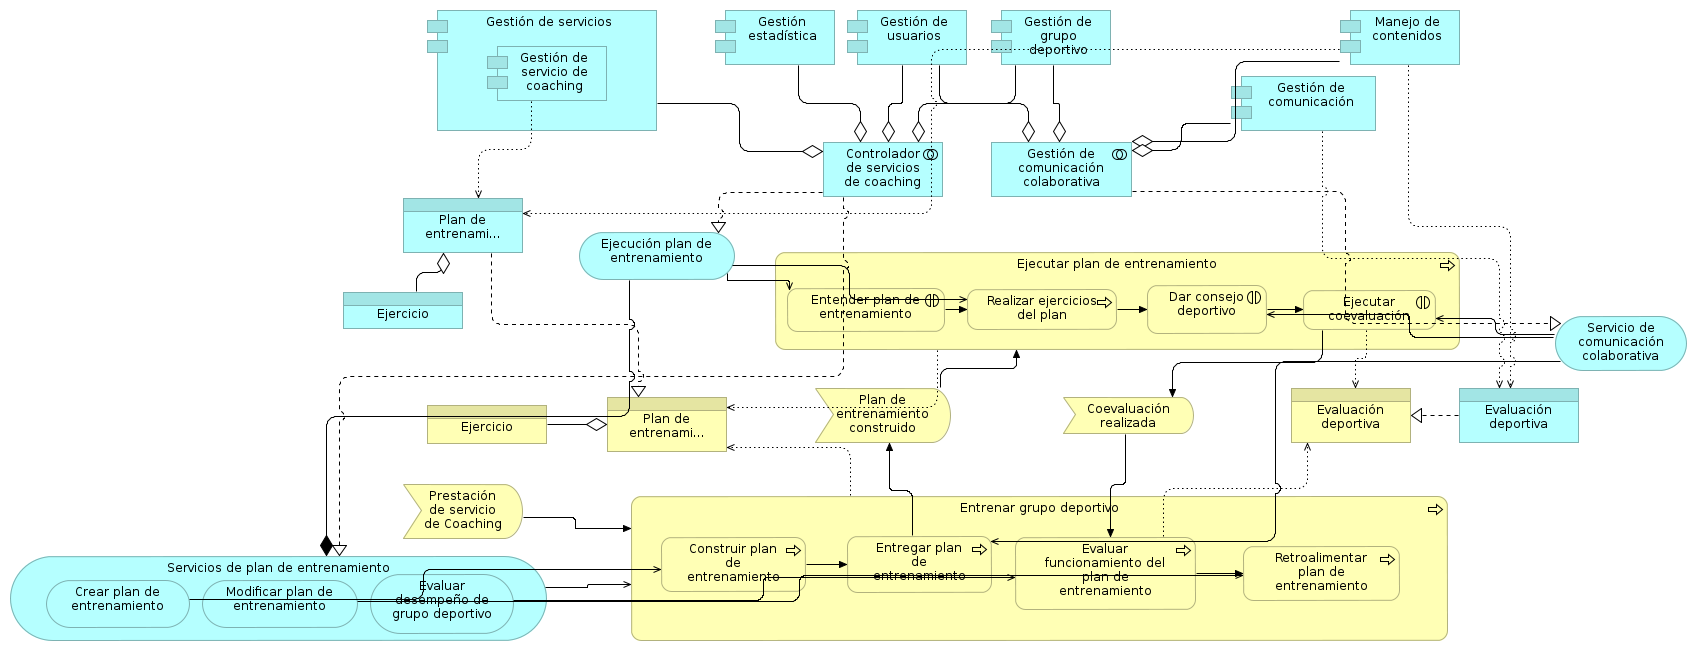
\includegraphics[width=11cm]{./imagenes/Archimate/vistas/application_usage/entrenamientodeportivo.png}
    \caption{Entrenamiento Deportivo}
    \label{fig:au_entrenamiento_deportivo}
    \textbf{Fuente:}  Autores
  \end{center}
\end{figure}

Para el soporte de los servicios proporcionados por el SNS, son utilizados componentes de estadística, de gestión de usuarios y de grupos deportivos, así como también de comunicación y de manejo de contenidos para la evaluación de los entrenados y la ejecución del plan de entrenamiento por parte de los mismos. Hay un último componente de aplicación que es el de gestión de servicio de coaching, el cual realiza los servicios relacionados con el plan de entrenamiento y que, a su vez, está compuesto en el componente de gestión de servicios ya que éste entrenamiento deportivo es visto en la red social como otro servicio prestado a los actores que ella interactúan.